\chapter{Introduction}
\label{intro}

In this chapter, diabetic retinopathy and diagnosing diabetic retinopathy is discussed. The chapter contains the potential benefits of automated detection of diabetic retinopathy and eye fundus images.  (Bu kisim degisecek - research question vs ekle)

\section{Diabetic Retinopathy}


\subsection{Structure of Eye}

\begin{figure}[t]
\caption{Structure of eye \citep{WikipediaEN:AFM}}
\label{structureOfEye}
\centering
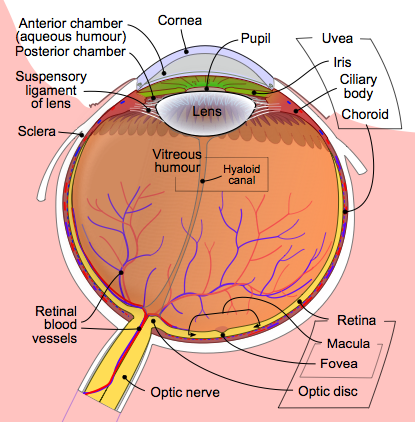
\includegraphics[width=0.8\textwidth]{Figures/structure_of_eye}
\end{figure}

As \citet{hughes2004anatomy} said our sense organ eye,"window to the soul", is interest of lots of disciplines. (Buraya baglanti ekle) As seen on Figure \ref{structureOfEye} light reflected from an object enters eye in the order cornea, pupils and lenses \citep{falt2012modern} and focused on retina. Depends on bright or dark, or distance of object eye regulates changes like amount of lights enters eye or focus on objects with pupil and reshaping elastic lens \citep{kauppi2010eye}. (Buraya baglanti ekle)

\begin{figure}[t]
\caption{Cross-section of retina, choroid(C) and sclera(S) \citep{falt2012modern}}
\label{layersOfRetina}
\centering
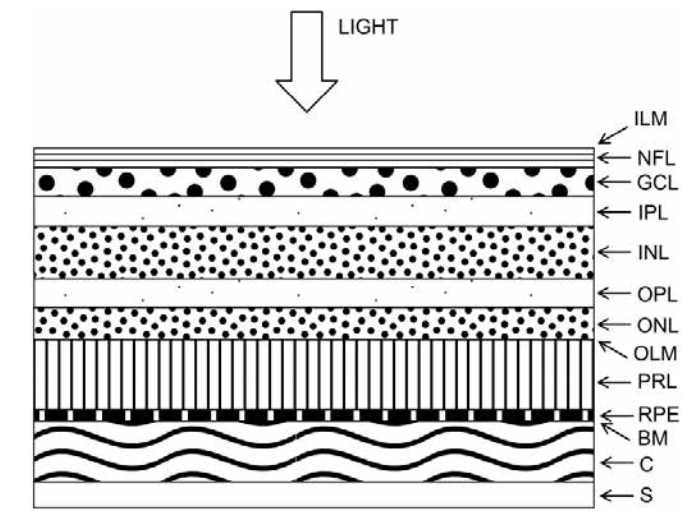
\includegraphics[width=0.8\textwidth]{Figures/layers_of_retina}
\end{figure}


In layers of retina, before transmitted to the brain via optic nerve for visual perception, the information in the light is processed \citep{kauppi2010eye}. These layers of retina are presented in Figure \ref{layersOfRetina}. The retina has 6 regions \citep{forrester2015eye}:

\begin{enumerate}
    \item Central retina
    \item Maculalutea
    \item Fovea centralis
    \item Optic disk
    \item Peripheral retina
    \item Ora serrata
\end{enumerate}

These anatomical parts of retina are represented on one of the colour fundus images in Messidor dataset \citep{mookiah2015application} in \ref{fundusPhotoRetina}. In this dissertation and as terms of retinal diseases, these are the terms I used. 

\begin{figure}[t]
\caption{Fundus Image \citep{mookiah2015application}}
\label{fundusPhotoRetina}
\centering
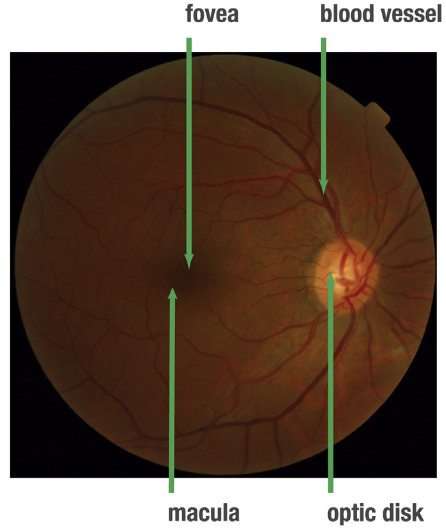
\includegraphics[width=0.8\textwidth]{Figures/fundus_photography_anatomical}
\end{figure}


\subsection{Diabetes Mellitus and Diabetic Retinopathy}
American Diabetes Association describes diabetes mellitus, which is a considered as global epidemic \citep{falt2012modern}, as "Group of metabolic diseases characterised by hyperglycemia resulting from defects in insulin secretion, insulin action, or both." \citep{national1979classification}. Diabetes mellitus can cause long term damages like on nervous system, kidneys, eye etc. Diabetic retinopathy(DR) is the most common eye disease as a result of damage on the retina of the eye triggered by diabetes mellitus and leading cause of vision loss in industrialised nations \citep{antal2014ensemble, stitt2013advances}. As a result of increasing number of diabetes mellitus patients, worldwide blindness caused by diabetic retinopathy will become more common if treatment of diabetic retinopathy will not improve \citep{wilkinson2003proposed}. Because diabetic retinopathy if not cured on early stages of disease, it can cause the complete loss of sight \citep{rocha2011points}. 

In early stages, patient does not have symptoms of diabetic retinopathy on their vision; the primary signs of DR are exudates \citep{nijalingappa2015machine}. In Figure \ref{visionOfDrAndNodr}, there is a scene from two different person; first one is normal vision and second one which has black areas on photo is the vision with advanced diabetic retinopathy \citep{NationalEyeInstitute}. 

\begin{figure}[t]
\caption{Same scene from normal vision person's eye[first] and person with advanced diabetic retinopathy[second]}
\label{visionOfDrAndNodr}
\centering
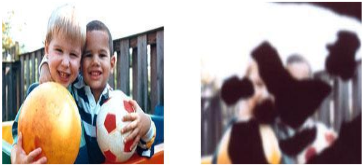
\includegraphics[width=0.8\textwidth]{Figures/vision_of_dr_and_nodr}
\end{figure}

Diabetic Retinopathy has divided two main stages depends on abnormal new vessels existence  \citep{tang2011inflammation, nijalingappa2015machine}; nonproliferative stages(NPDR) which are early stages of DR and advanced stage of DR, proliferative stage(PDR). 
During NPDR, DR progress in 3 stages:

    \begin{enumerate}
        \item Mild NPDR
        \item Moderate NPDR
        \item Severe NPDR
    \end{enumerate}


\citet{NationalEyeInstitute} and \citet{wilkinson2003proposed} define these 4 stages of DR as follows:
\begin{enumerate}
        \item \textit{Mild NPDR:} It is the earliest stage of DR. In retinal capillaries, small changes starts. The smallest detectable abnormalities of DR, only \textbf{microaneurysms (MA)} are detectable as small red dots.
        \item \textit{Moderate NPDR:} It is the second stage of DR. Blood vessels may start to lose blood circulation ability and/or swell and distort. \textbf{Haemorrhages (HA)} starts to appear. These changes may cause diabetic \textbf{macular edema (DME)}.  
        \item \textit{Severe NPDR:} Vessel blockage is increased in this stage; retina starts to trigger body to develop new vessels for supplying nutrition and oxygen to suffering areas. But these vessels are fragile and thin. \textbf{Intra-retinal microvascular abnormalities (IRMA)} are also sign of this stage. 
        \item \textit{PDR:} In the PDR stage, \textbf{neovascularisation} which is the development of these new fragile vessels starts. These fragile vessels  are dangeruous because they can cause sudden vision loss. \textbf{Soft exudates (cotton wool spots)} are visible in PDR. 
\end{enumerate}


Hard Exudates(HA), Haemorrhages (HA), microaneurysms (MA) presented on Figure \ref{AbnormalitiesFundusImage}

\begin{figure}[t]
\caption{Hard Exudates(HA), Haemorrhages (HA), microaneurysms (MA) abnormalities on Fundus Image \citep{kekre2013hybrid}}
\label{AbnormalitiesFundusImage}
\centering
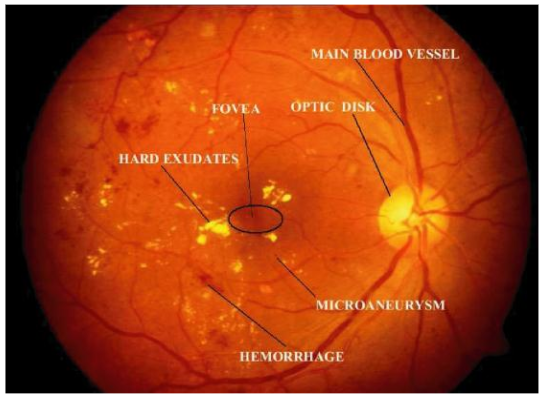
\includegraphics[width=0.8\textwidth]{Figures/retina_abnormalities}
\end{figure}

\subsection{Diagnosing Diabetic Retinopathy}

In this section, I explain how diabetic retinopathy diagnoses and main methods for diagnosing DR.

Early diagnosis of DR is very important to prevent vision loss on diabetes mellitus patients \citep{mankarautomatic}. Diagnosing DR is very difficult if diabetes mellitus is not suspected on patient. DR is not visible on blood samples. These make DR a deceptive disease \citep{kauppi2010eye}. To detect DR, patient should take extensive eye exam. \citet{kauppi2010eye} grouped these examinations as follows:
\begin{itemize}
    \item Clinical eye examination,
    \item Eye fundus photography,
    \item Fluorescein angiography,
    \item Optical Coherence tomography (OCT).
\end{itemize}
Since 1980s, eye fundus photography is available and it made opthalmoscopy the most commonly used examination method, if available, for diagnosis of DR \citep{wendt2005screening}. Eye fundus photography lets to save the data and it helps ophthalmologists examine the image later \citep{hutchinson2000effectiveness}. 

\citet{rocha2011points} grouped diagnosing anomalies of DR in following titles and they added that diagnosing DR-non DR is recently becoming popular approach for diagnosing DR:  
\begin{enumerate}
    \item \textbf{Detection of blood vessels:}  Because eye is the only place where blood vessels can directly be observed only on human body, it is unique. DR causes changes on vascular conditions in eye. Detection of any changes in the blood vessels is a way to diagnose DR on retinal fundus images. \citet{mendonca2006segmentation}
    \item \textbf{Detection of hard exudates:} Retinal oedema is the major cause of vision loss during DR progress. Existence of hard exudates, addresses the presence of retinal oedema \citep{singer1992screening} which helps ophthalmologists diagnosing and follow-up of DR \citep{garcia2009neural}.
    \item \textbf{Detection of microaneuysms:} In earliest stage of DR, microaneurysms, and hemorrhages are visible \citep{doi:10.1056/NEJMra021678}. Hard exudates and cotton wool spots are not able to detect in early stages of DR \citep{navarro2016automatic}. Because it is easier to prevent DR in earlier stages, detecting microaneuysms are important.
    \item \textbf{Detection of hemorrhages:} Hemorrhages are visible in early stages of DR like microaneuysms but this anomaly is more visible on advanced stages of DR; the more hemorrhages means that the more retina damage progression. In literature, the following approaches are presented for detection of hemorrhages \citep{rocha2011points}:
    \begin{enumerate}
        \item Detection of blood vessels
        \item Detection of blood vessels with hemorrhages
    \end{enumerate}
\end{enumerate}

Algorithms and results used for these detections can be found in Chapter~\ref{related_work}.




\subsection{Screening Diabetic Retinopathy}

Can be extracted???? 


\section{Background (?)} 

\subsection{Restrictions}
\subsection{Contributions}



\section{Research Question(s)}
In this work we try to answer the following research questions:

\begin{itemize}
    \item Can signs of DR can be detected automatically by using machine learning algorithms especially by using deep learning methods?
    \item Can we detect signs of DR in a dataset by using another dataset's trained model?
    \item Will using deep learning on the task of detection of DR open new research directions in this area? 
\end{itemize}
\section{Motivation}
According to Natinal Eye Institute only in USA around 40-45\% of people having diabetes were diagnosed with diabetic retinopathy. Besides, nearly 35\% of people having diabetes in worldwide have DR and 1 in 10 will have a vision threatening form of the disease \citep{yau2012global}. According to a recent work diabetic retinopathy effects almost 4\% of people of Europe also \citep{nentwich2015diabetic}. Therefore, it is essential to detect the signs of DR in the early stages. The process to detect the signs of diabetic retinopathy needs trained technicians to work on the eye images, analyse. Our main motivation is to make this process automatic by using convolutional neural networks.
\section{Aims and Objectives}
As clearly explained in the previous sections, our main aim and goal is the automatic detection of the early signs of DR by using one of the widely used deep learning methods, convolutional neural networks. We look for the results of using a big dataset as training data and other available public datasets as test datasets. 
\section{Reports Structure}
The structure of this work is as follows: first we review the ralated work in the next section, then we explain our methodology and give experimental setup and the result of the experiments. Finally we conclude our work. 
